\chapter{Methods}
\label{chapter:methods}

In this chapter we begin by first describing the common approaches followed by researchers for a variety of energy consumption experiments, their advantages and disadvantages. Then we present the approach we followed for our study and its justification.
\section{Common Approaches}
\label{section:commonappraoches}
One approach for estimating energy consumption of a given network is by employing actual power meter to measure the power drawn by involved network and computing components. A good example for such case is the measurement that Fan and his team conducted~\cite{DBLP:conf/isca/FanWB07}. In this study the authors have managed to monitor power consumption of several thousand of servers over a period of six months on real live workload. Mahadevan et al.,~in~\cite{DBLP:conf/networking/MahadevanSBR09}, have also done a similar power measurement on a production environment for studying power consumption behavior of networking devices such as switches and routers. If the measurements are done correctly, this approach produces the most real picture of the network under investigation compared to the other two approaches that we will discuss in subsequent paragraphs. However, this approach has certain inherent drawbacks. First, real production networks might not be available for experimentation. Even if they become available, the transient and varying nature of the production environment makes it hard to repeat the experiments. Second, we have little or no control over factors affecting the measured power consumption. We do not have the privilege of injecting or modifying the traffic or the workload in order to test different experimental hypothesis. To have a full control we need another approach. 

Experimental testbed is another approach that researchers have used to study power consumption characteristics of different computing and networking devices. In this approach first a separate network is setup and configured solely for the purpose of conducting experiments. Then researchers make measurements by manipulating factors that affect power consumption according to the hypothesis that they want to test. Unlike the previous one, this approach offers greater flexibility over the experimental parameters. In the power measurement study scenario that we are discussing, the researcher can change parameters such as traffic rate, packet size, inter-packet time interval and transmission protocol used (TCP/UDP). Sivaraman et al.~in~\cite{Sivaraman} have setup experimental testbed for determining per-packet processing and per-byte receipt, storage, queuing, and transmission power consumption. The experiment setup involved hardware-based traffic generator (which gives fine grain control over parameters such as the packet size, inter-packet interval and data rate), NetFPGA\footnote{http://www.netfpga.org/} experimental router and digital oscilloscope for measuring the power draw of the NetFPGA router. A similar experiment but with commercial switches of different vendors is explained in~\cite{DBLP:journals/comcom/SivaramanRZSVMR14}. The primary advantages of this approach is that the researcher can have full control over the experimental parameters provided by the tools involved in the testbed and experimental result can also be very accurate. The first disadvantage though is that it can easily become very expensive when we want to experiment on large-scale level. The second disadvantage is that experimenting on different scenario might require considerable reconfiguration and even a completely new testbed, which apart from limiting the flexibility, it can also be very costly, time and effort consuming. We need an approach which overcome these shortcomings. That is, we need an approach which gives full control over the experiment, which is reasonably accurate, less expensive and very flexible. 

Simulation is the most widely used approach in computer network research~\cite{DBLP:conf/icc/WeingartnerLW09}. It has several advantage compared to the other two approaches mentioned before. First, it makes it relatively easy, for instance, the study of the performance of non-existing network protocol or algorithm. One can propose and validate, by simulation experiment, a new energy-aware routing protocol or algorithm for wired or wireless networks. This is what Swain et al.~\cite{DBLP:conf/aina/SwainHC10} did in their new energy-aware routing protocol proposal for wireless sensor networks. Second, though it depend on the design of the particular simulator used, in general, simulation approach allows running large scale experiments that involve hundreds and thousands of nodes with less effort and cost compared to the other two approaches. In~\cite{DBLP:conf/wowmom/OrgerieLLL11} and~\cite{DBLP:conf/cloudnet/CorneaOL14}, the NS-3 module, ECOFEN, is used to simulate energy consumption of large-scale networks with nodes more than 600 and 1000, respectively. In~\cite{DBLP:journals/tjs/KliazovichBK12} Kliazovich et al.~studied energy consumption of data center networks with two-tier and three-tire architectures that encompasses 1536 nodes. Third, in simulation scaling does not incur monetary cost, though it is limited by performance factors such as runtime and memory usage~\cite{DBLP:conf/icc/WeingartnerLW09}. Fourth, the researcher has great flexibility and full control over the simulation experiment. Finally, simulators makes output data management extremely easy by providing mechanisms such as logging, tracing and visualization~\cite{ns3,DBLP:journals/jpdc/CasanovaGLQS14}.  

Though simulation experiment has quite a lot of advantages over experiments done on production environment or experimental testbeds, it faces one big challenge, accuracy. In the process of approximating the real network phenomenon in the simulation model, some less significant concepts are abstracted away, for instance, to reduce complexity or to gain performance improvement, which results in unavoidable loss of accuracy. However, in other instances the models used in a given simulator might fail to correctly capture the simulated real network phenomenon. In~\cite{DBLP:journals/tomacs/VelhoSCL13} the authors demonstrated incorrect modelings found in popular simulators such as OptorSim, GridSim and CloudSim. Therefore, (in)validating the correctness of a simulator is important task that should be undertaken before any simulation experiment for two related reasons. Either to know the boundaries within which the simulator used produce reasonably accurate results, or to know if the simulator produce the expected or the correct result. The validation can be done either by comparing the output of the simulator against accurate measurements obtained from real networks or by comparing the output against another simulator whose accuracy is already known~\cite{DBLP:books/daglib/0076234}.
\section{Our Approach}
\label{section:ourapproach}
The goal of this study is to investigate the accuracy and scalability of flow-level models, as compared to packet-level models, in estimating energy consumption of large-scale distributed networks. To achieve this goal, we first search literature to find and propose a suitable flow-level model. Second, we implement the model in SimGrid. Finally, we run different experiments to test the accuracy and the scalability of the implemented flow-level model by comparing it against a packet-level model. For our experiments, we chose the simulation approach among the three alternatives discussed above. 

Before describing the details of our approach, let us first justify why we end up with the relatively complex method shown in Figure~\ref{fig:approach}. There is experimental test-bed (Grid'5000\footnote{https://www.grid5000.fr/mediawiki/index.php/Grid5000:Home}) in France that we have access to. Grid'5000 is experimental test-bed specifically designed for studying large-scale distributed networks~\cite{DBLP:journals/ijhpca/BolzeCCDDJJLLMMNPQRTT06}. However, we could not used it for our purpose (i.e., for studying large-scale flow-level relationship of power consumption and traffic) as the network devices are not equipped with power meters accurate enough (current power meters on Lyon site of Grid'5000 provide one measurement per node and per second). As a result, we opted to use a packet-level simulator with power consumption models obtained from literature. Subsequent paragraphs describe the specific steps we followed in our approach.

As we have discussed in Chapter~\ref{chapter:background}, SimGrid already have energy consumption model for CPU which corresponds to the computing part of a given large-scale network. What we wanted to add is energy consumption model for communication components such as switches and routers. Therefore, the initial task in our approach is to study literatures (\circled{A} in Figure~\ref{fig:approach}) in order to find and propose a model which describe the power consumption characteristics of communication equipments such as switches and routers. Our search returned the linear relationship that we have described in Equation~\ref{eq:2.2}~\cite{Sivaraman,DBLP:journals/comcom/BeisterDAK14,DBLP:conf/networking/MahadevanSBR09,DBLP:conf/sigcomm/MahadevanBS10}. This equation tells us that the power consumption of a network equipment constitutes the idle and dynamic components. The idle power consumption represents the power drawn by the equipment while it is on but with no traffic. The dynamic consumption, on the other hand, represent the additional power drawn due to network traffic. The next task (\circled{C} in Figure~\ref{fig:approach}) is to implement this linear model for SimGrid and (in)validate its accuracy against ECOFEN module (\circled{D} in Figure~\ref{fig:approach})~\cite{DBLP:conf/wowmom/OrgerieLLL11,DBLP:conf/cloudnet/CorneaOL14}. This task is done iteratively by switching between model implementation and accuracy validation. The final task (\circled{G} in Figure~\ref{fig:approach}) is to show the scalability of the implemented flow-level model against the existing packet-level model in ECOFEN. For this, we designed and run two kinds of experiments (\circled{E} and \circled{F} in Figure~\ref{fig:approach}), one for speed and one for memory usage. 

The purpose of the accuracy and the scalability experiments shown in \circled{D} and \circled{G} in Figure~\ref{fig:approach} is to test our \emph{hypothesis}, which states: \emph{flow-level energy consumption models can give reasonably accurate estimation and they can also be significantly more scalable than packet-level models}. 

We chose to use ECOFEN as packet-level simulator to compare the accuracy and performance of the implemented model for two primary limitations that exist in the other alternative simulator, GreenCloud~\cite{DBLP:journals/tjs/KliazovichBK12}. The first limitation is that GreenCloud is designed for a  cloud computing environment. This is in contrary to one of SimGrid's main design principles, versatility~\cite{DBLP:journals/jpdc/CasanovaGLQS14}. ECOFEN, on the other hand, is not tied to one particular large-scale networking paradigm, therefore, suits more for our purpose. The second limitation of GreenCloud is that it is build on top of currently obsolete NS-2 simulator. In comparison, though ECOFEN was also initially built as NS-2 simulator module, currently it is rewritten for NS-3~\cite{DBLP:conf/cloudnet/CorneaOL14}. One of the major advantage of using NS-3 over NS-2 is that NS-3 performs considerably better in both runtime and memory-usage metrics~\cite{DBLP:conf/icc/WeingartnerLW09}.

In the accuracy-validation and scalability-comparison experiments mentioned in our approach, we are comparing the newly implemented flow-level model in SimGrid simulator against another packet-level simulator model implemented in ECOFEN module. This simulator-to-simulator comparison is valid only if the later simulator model, against which the new implementation is to be validated, is known to be accurate. However, we could not find any information that tell us the accuracy of the ECOFEN module. Therefore, we designed a validation experiment (\circled{B} in Figure~\ref{fig:approach}) for ECOFEN as described in the next section. 
\begin{figure}[ht]
	\begin{center}
		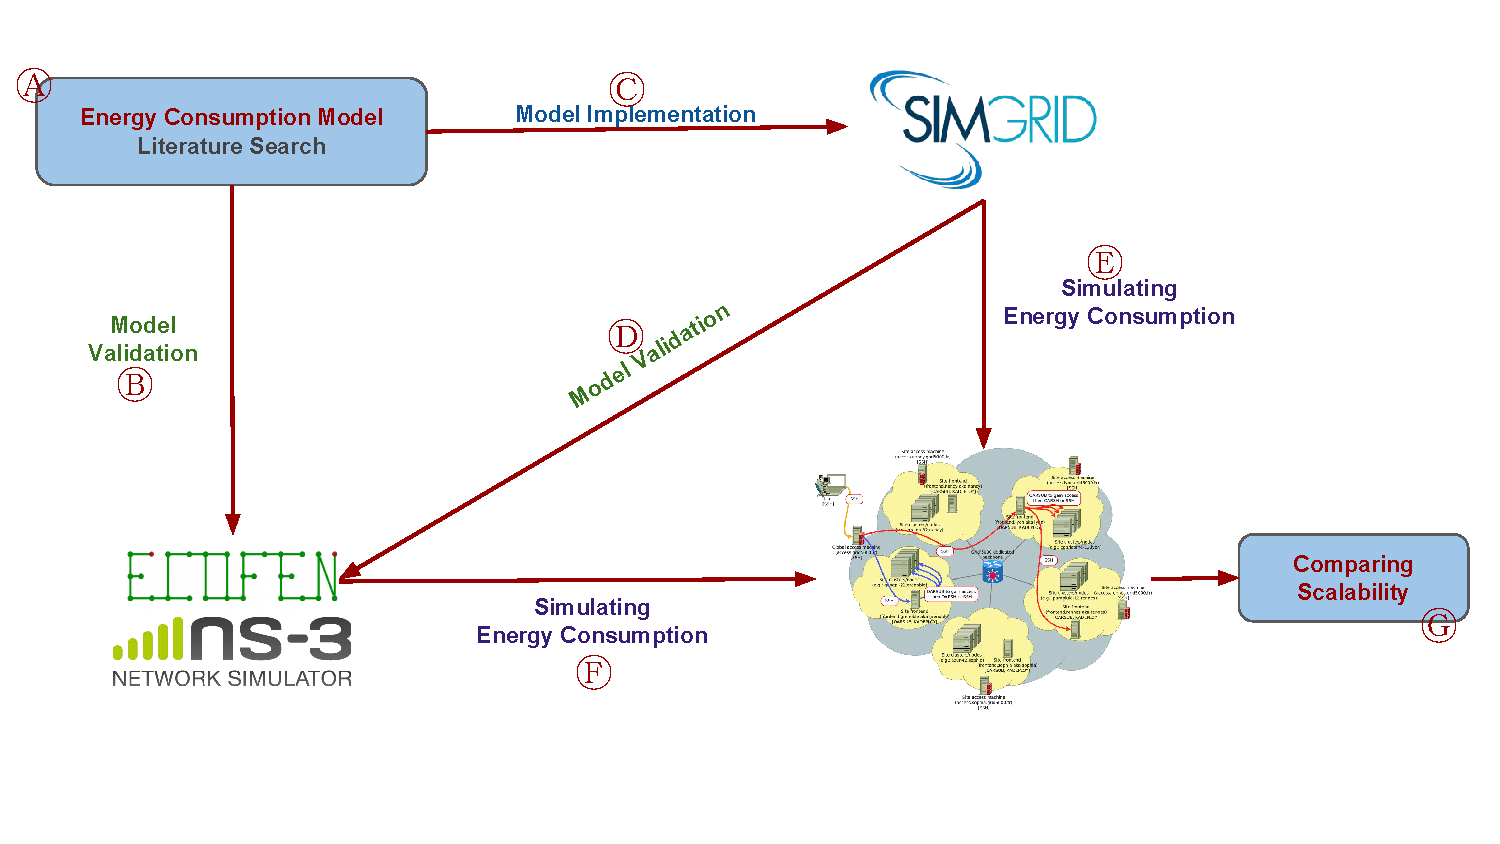
\includegraphics[width=13cm]{images/approach.pdf}
		\vspace*{-1.0cm}
		\caption{Summary of the experimental method we followed in this study}
		\label{fig:approach}
	\end{center}
\end{figure}
\section{Validating ECOFEN}
ECOFEN has three models with names \emph{basic}, \emph{linear} and \emph{complete} that we have discussed in Section~\ref{section:relatedsimulator} of Chapter~\ref{chapter:background}. Both the \emph{linear} and \emph{complete} models can produce values of power consumption as a function of traffic. The  \emph{basic} model, on the other hand, produces power consumption values based on the ON or OFF state of a node, it does not consider network traffic. Therefore we describe the validation experiments for both the \emph{linear} and the \emph{complete} models in this section. 
 
The basic procedure for the validation experiment is first to simulate, using ECOFEN, power consumption in response to traffic sent or received and then to compare the results against data obtained from literature where actual measurement is conducted.

\subsubsection{Validating the Linear Model}
In the work of Sivaraman et al.~\cite{Sivaraman} we can find the result of a power consumption experiment that is shown in Figure~\ref{fig:powervsdatarate1}. The figure displays the linear relationship that exist between traffic volume (in Mbps) and power consumption (in watts) for a fixed packet sizes of 100, 576, 1000, and 1500 bytes. Furthermore, in the figure, the linear fit equations (models) for each of the packet sizes are also displayed. 

The authors intention in this experiment is to determine values of the per-byte and the per-packet processing energy consumption, however, our intention is to use the per-byte energy consumption value that they have experimentally determined and to use it in ECOFEN to get power consumption values for a given volume of traffic. Then compare the results we obtained with the linear fit models that are shown in Figure~\ref{fig:powervsdatarate1}. The linear fit equations shown in Figure~\ref{fig:powervsdatarate1} are derived from actual power measurements.

In their experiment, the authors used three kinds of hardware devices: (1) NetFPGA router card that has four 1 Gbps Ethernet ports, (2) IXIA hardware traffic-generator for generating packets with the desired packet-size and data-rate, and (3) high-fidelity oscilloscope for measuring the power consumed by the NetFPGA card as a consequence of the packets send or received. 

\begin{figure}[ht]
	\begin{center}
		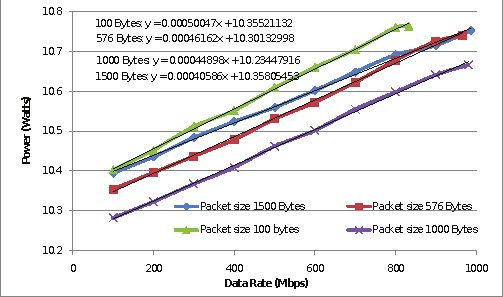
\includegraphics[width=13cm]{images/powervsdatarate1.pdf}
		\caption{Power consumption vs data-rate for fixed packet size from~\cite{Sivaraman}.}
		\label{fig:powervsdatarate1}
	\end{center}
\end{figure}

The linear model of ECOFEN module accepts energy consumption values for the idle state of a simulated network interface card (NIC) and the per-byte processing. The underlying NS-3 platform, in addition, provides us with more parameters such as packet-size and data-rate, which among other parameters, enable us to have full control over the generated traffic.

In this validation experiment we wish to simulate the experiments conducted by Sivaraman et al.~as closely as possible. With this in mind, we setup, in our NS-3 simulation script, a three node simple network with first and third nodes connected to the second node. All the three nodes are connected to each other by links that have maximum bandwidth capacity of 1 Gbps and delay of 10 ms. 

We got the idle consumption values for each of the packet-size models shown in Figure~\ref{fig:powervsdatarate1} by setting the x component (the data rate value) of the equations to zero and for a per-byte processing energy consumption value we used 3.4 nJ. This is the value that the researchers experimentally determined. 

For the generated traffic volume in the simulation, we used uniform random number generator provided by NS-3 in order to get integer values between 1 and 1000. Our NS-3 script, in addition to packet-size and data-rate values, also requires number of packets to be send and also inter-packet interval time values. These values are derived from packet-size and data-rate parameters. 

Since there might be unexpected results, for instance, due to wrong network configuration, we have employed NS-3's FlowMonitor module to monitor the actual traffic transfered in the simulated network. Using this flow monitoring module, we have confirmed if all the traffic generated by the sending end are also received at the receiving end. We have also used this module to compute the actual traffic rate (throughput) both at the receiving and the sending ends as shown in Equation~\ref{eq:3.1} and Equation~\ref{eq:3.2} in Chapter~\ref{chapter:environment}.

Finally, we set the remaining simulation environment configuration settings such as starting and stopping time and then run the experiment 40 times, each time with different run value for the random number generator. The result obtained is depicted in Figure~\ref{fig:linear}. In the graph the expected power consumption values from the linear fit models shown in Figure~\ref{fig:powervsdatarate1} along with the simulated values for each of the packet sizes (100, 576, 1000, and 1500 bytes) are displayed.

Visually, the simulated and the expected values seem to agree very well, even though the gap between them starts to grow slightly larger (especially when the packet size is 100 bytes) for larger data-rates. In order to be more sure, we run unpaired t-test statistical test using the produced data. The summary of this test is shown in Table~\ref{table:linearttest}. 

The 95\% confidence interval values shown in Table~\ref{table:linearttest} of difference in mean between the measured and simulated values are very close to zero and in fact zero is also one of the values. The P-values are also confirming the same thing, the null hypothesis that the difference in mean between the simulated and the expected values is zero is not rejected. 
\begin{figure}[ht]
	\begin{center}
		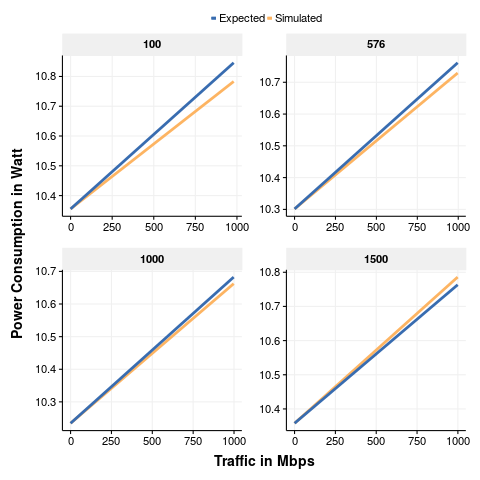
\includegraphics[width=13cm]{images/expectedvssimulatedlinear.png}
		\caption{Power consumption vs data-rate comparison between expected (or measured) values (in red color) and simulated values (in light blue color) for a fixed packet size of 100, 576, 1000, and 1500 Bytes}.
		\label{fig:linear}
	\end{center}
\end{figure}
\begin{table}
	\begin{tabular}{|>{\centering\arraybackslash}m{1.3cm}|>{\centering\arraybackslash}m{4.2cm}|>{\centering\arraybackslash}m{2.1cm}|>{\centering\arraybackslash}m{2.1cm}|>{\centering\arraybackslash}m{1.3cm}|} 
	    \hline 
		\textbf{Packet Size} & \textbf{Confidence Interval of difference in mean} & \textbf{Mean of Expected} & \textbf{Mean of Simulated}& \textbf{P-Value}\\ 
		\hline 
		 100 &	[-0.027, 0.110] &         10.640 &         10.599 &  0.230\\
		\hline
		 576 &[-0.039, 0.082]&        10.544 &          10.523 &  0.480\\ 
		\hline
		 1000&	[-0.043, 0.073] &         10.466 &          10.451&0.6131\\ 
	    \hline	 
	     1500&	[-0.062, 0.048] &         10.566 &          10.573&  0.796\\ 
	    \hline
	\end{tabular} 
	\caption{Unpaired t-test results for simulated and measured power consumption values for ECOFEN's linear}
	\label{table:linearttest}
\end{table}

The conclusion in this validation test is that the linear model of ECOFEN is accurate in predicting the power consumed by NetFPGA router for a given volume of traffic. 

\subsubsection{Validating the Complete Model}
Roughly, in this validation experiment, we have used the same experimental configuration and procedure as that of the linear validation experiment that we have described in the previous section. Therefore, in this section our focus is more on the result than on the configuration.

One of the main difference between the complete and the linear model of ECOFEN is that the complete model distinguishes between the received and sent bytes. Which means that different energy consumption values can be assigned to bytes based on the direction of transfer. The linear model, on the other hand, assigns same value for both. The other main difference is that the complete model considers the packet processing energy consumption cost both for the sent and received packets. 

Sivaraman et al.{\ }\cite{Sivaraman} also conducted experiments to determine energy consumption values for per-byte receive or transmit and per-packet processing. The experimentally determined values for per-byte receive is 1.3 nJ, for per-byte transmit is 2.1 nJ, and for per-packet processing is 197.2nJ. 

We have slightly modified the NS-3 script that we have used in the previous section to make it suitable for this experiment. Now we have configured our script for the ECOFEN's complete model to use energy consumption values for per-byte receive or send and per-packet processing. Further more, we have upgraded the link capacity between the nodes from 1 Gbps to 2 Gbps. Finally, we set the traffic rate in terms of packets per second in the sending end and in terms of Mbps in the receiving end in order to comply with the experiments done by mentioned authors. The results for the sending and receiving are is shown in Figure~\ref{fig:sending} and Figure~\ref{fig:receiving}, respectively. The linear fit models we have used for this validation experiment are also available in \cite{Sivaraman}. There is only one linear fit model (for packet size 1000 bytes) for the sending end and there are three for the receiving end.   
\begin{figure}[ht]
	\begin{center}
		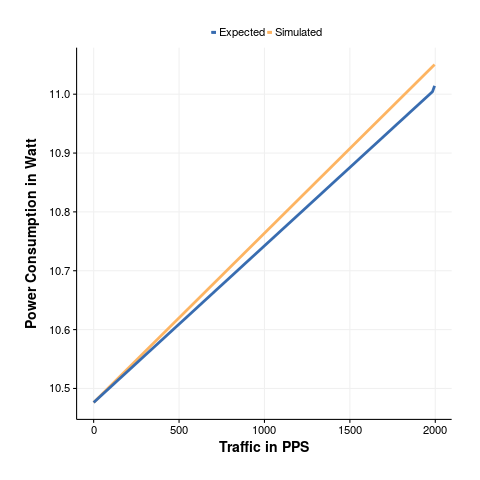
\includegraphics[width=11cm]{images/expectedvssimulatedsending.png}
		\caption{Power consumption vs data-rate comparison between expected (or measured) values (in red color) and simulated values (in light blue color) for a fixed packet size of 1000 Bytes for the sending end}
		\label{fig:sending}
	\end{center}
\end{figure}
\begin{figure}[ht]
	\begin{center}
		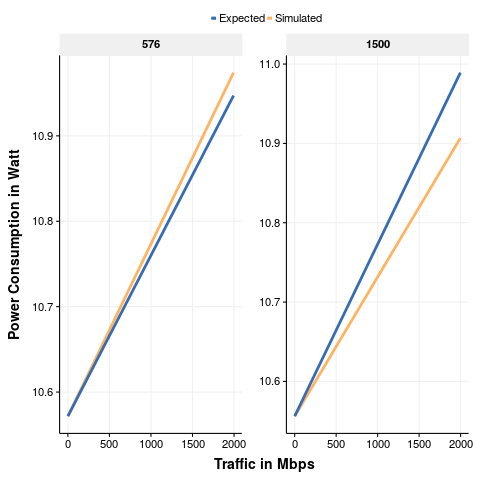
\includegraphics[width=11cm]{images/expectedvssimulatedreceiving.png}
		\caption{Power consumption vs data-rate comparison between expected (or measured) values (in red color) and simulated values (in light blue color) for a fixed packet size of 576 and 1500 Bytes for the receiving end}
		\label{fig:receiving}
	\end{center}
\end{figure}
Table~\ref{table:complettest} shows the unpaired t-test result for one packet-sizes in the transmitting side (Tx) and for two packet-sizes in the receiving side (Rx). 
\begin{table}
	\begin{tabular}{|>{\centering\arraybackslash}m{1.3cm}|>{\centering\arraybackslash}m{0.7cm}|>{\centering\arraybackslash}m{3.9cm}|>{\centering\arraybackslash}m{2.1cm}|>{\centering\arraybackslash}m{2.1cm}|>{\centering\arraybackslash}m{1.2cm}|} 
		\hline 
		\textbf{Packet Size} & End &\textbf{Confidence Interval of difference in mean} & \textbf{Mean of Expected} & \textbf{Mean of Simulated}& \textbf{P-Value}\\ 
		\hline 
		576 &	Rx&[-0.067, 0.039]&         10.770 &          10.784&   0.598 \\
		\hline
		1500&	Rx&	[-0.010, 0.095] &        10.778 &         10.736& 0.114\\ 
		\hline
		1000&	Tx&	[-0.096, 0.053] &        10.750 &         10.773 & 0.560 \\ 
		\hline	 
	\end{tabular} 
	\caption{Unpaired t-test results for simulated and measured power consumption values for ECOFEN's complete model}
	\label{table:complettest}
\end{table}

Again in this case the 95\% confidence interval values shown in Table~\ref{table:complettest} of difference in mean between the measured and simulated values are very close to zero and in fact zero is also one of the values. The P-values are also confirming the same thing, the null hypothesis that the difference in mean between the measured and the simulated values is zero is not rejected. 

The conclusion from this validation experiment is also the same as the previous one, the ECOFEN's complete energy consumption model accurately predicts power consumed by NetFPGA router for a given volume of sent or received traffic.  

 

